\documentclass[pflichtenheft.tex]{subfiles}

\begin{document}

\chapter{Graphische Benutzeroberfläche}
Auf den Endgeräten wird eine Grafische Benutzeroberfläche angezeigt. Diese wird soll sich je nach Endgerät nur im verfügbaren Platz aufgrund der Größe der Displays unterscheiden, nicht aber in Funktionalität.

Der Nutzer soll GUI Instrumente anzeigen und ausblenden können. Zu den GUI Instrumenten gehören sowohl Dashes mit Realtime Info, als auch Graphen, die Aufzeichnungen von Daten in einem längeren Zeitraum visualisieren. Einige GUI Elemente sind invariant, also werden stets angezeigt.


\section{DashBoard}

Auf dem Dashboard werden verschiedene Anzeigeelemente dargestellt. Welche diese sind lässt sich einstellen. 

\begin{figure}[h]
  	\begin{center}
 		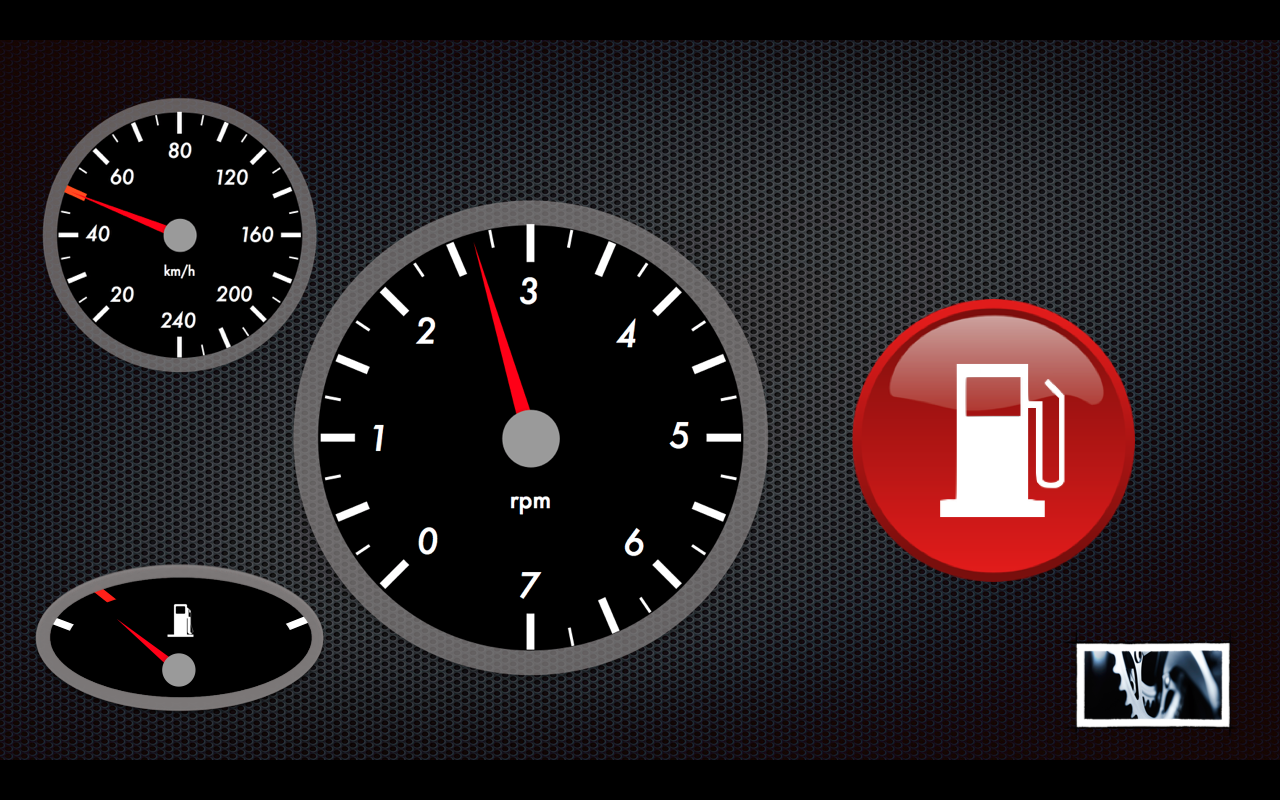
\includegraphics[width=\textwidth]{Images/GUI-Dash.png}
  		\caption{Das normale Dashboard.}
  	\end{center}
\end{figure}


\section{Dashboard mit Statistik}

Weitere mögliche Anzeigeelemente sind Graphen auf denen Statistiken eines Wertes angezeigt werden können. Es 
\begin{figure}[h]
  	\begin{center}
 		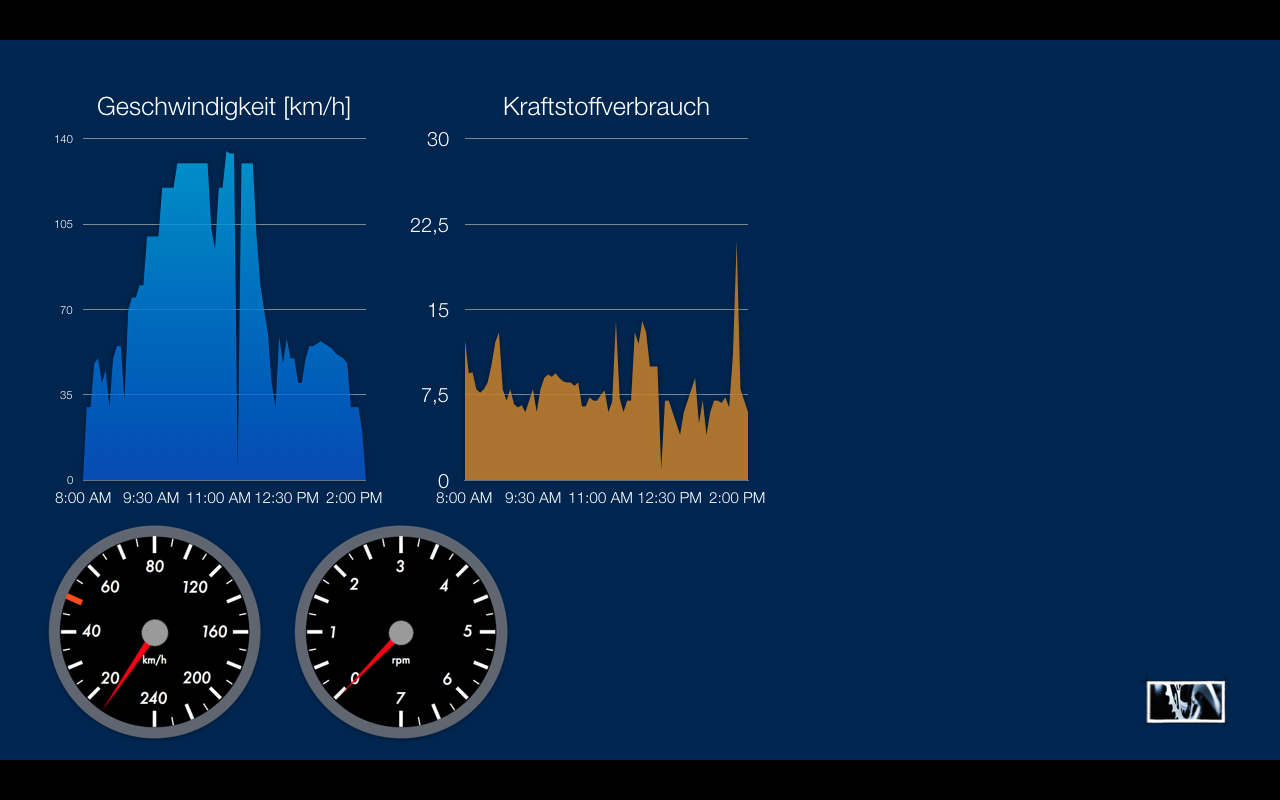
\includegraphics[width=\textwidth]{Images/GUI-DashStatistic.png}
  		\caption{Das normale Dashboard.}
  	\end{center}
\end{figure}

\clearpage
\section{Tabelle}

Die Tabelle, kann in verschiedenen Anzeigen genutzt werden. Die Tabellengröße, also die Anzahl der Spalten und Zeilen, ist variabel. Die Tabelle ist Scrollbar und ihre Zellen können mit verschiedenen Elementen, wie z.B. Bildern oder Text gefüllt werden. \\
Siehe z.B. ~\nameref{sec:Karte}

\begin{figure}[h]
  	\begin{center}
 		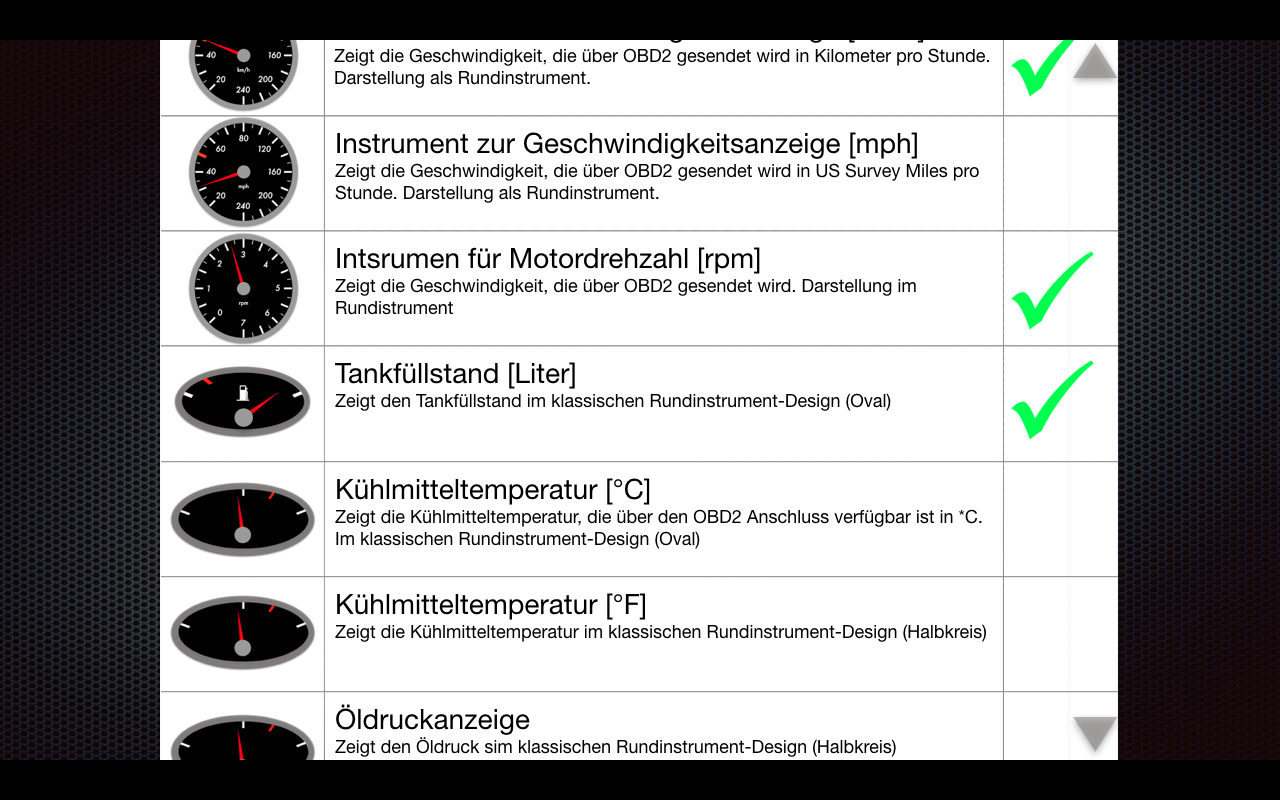
\includegraphics[width=\textwidth]{Images/GUI-Table.png}
  		\caption{Eine Tabelle}
  	\end{center}
\end{figure}

\clearpage
\section{Karte}
\label{sec:Karte}

Auf dieser Anzeige können links Vorschläge von Orten in der Nähe angezeigt werden. Rechts auf der Karte kann man diese Orte dann auf einer Karte, die die Umgebung anzeigt sehen. 

\begin{figure}[h]
  	\begin{center}
 		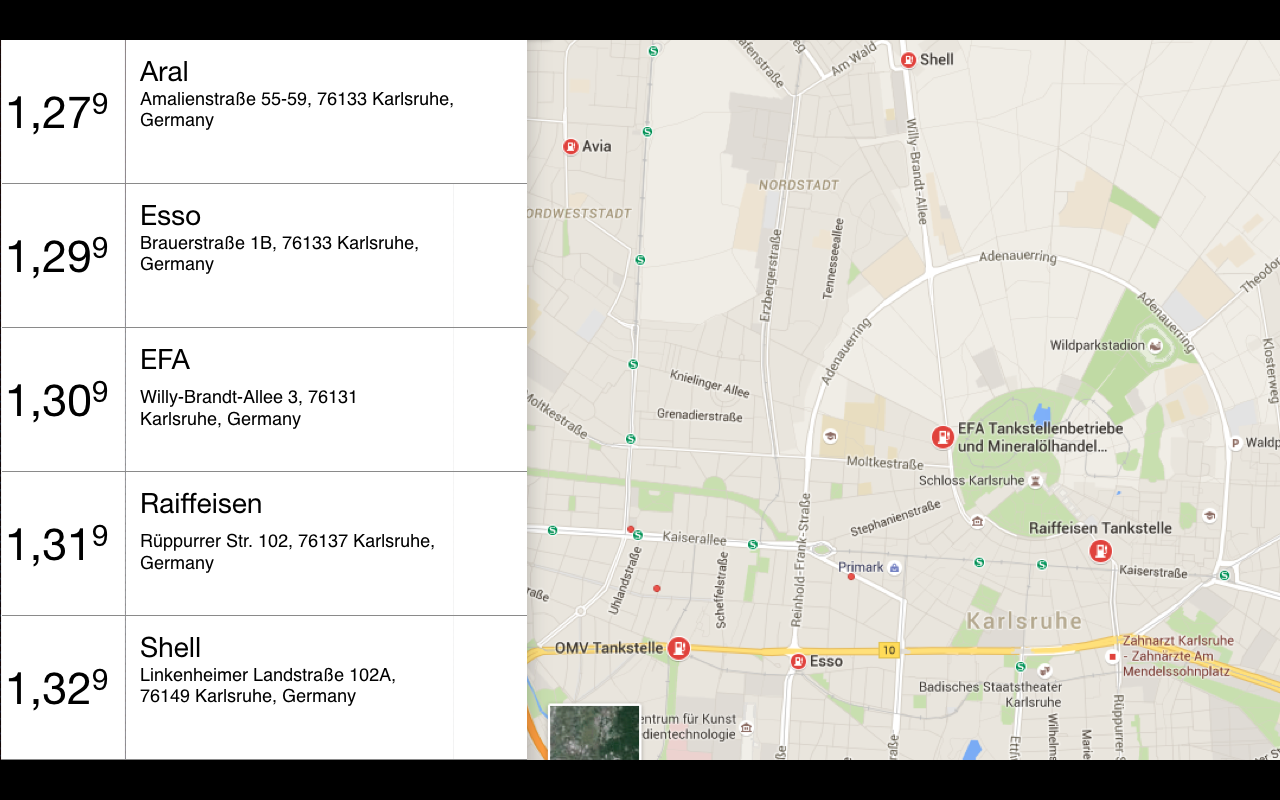
\includegraphics[width=\textwidth]{Images/GUI-Map.png}
  		\caption{Die Kartenanzeige mit einer Tabelle}
  	\end{center}
\end{figure}


\end{document}